\chapter{Κανονικοποίηση}
\label{appendix:Reg}
\paragraph{Διακύμανση - Πόλωση Μοντέλου}
Κατά την επιλογή του μοντέλου που θα χρησιμοποιήσουμε για μια εφαρμογή μηχανικής μάθησης, το βασικό δίλημμα μπροστά στο οποίο βρισκόμαστε είναι αυτό της πολυπλοκότητας της υπόθεσης. Το γεγονός πως προσπαθούμε να προσεγγίσουμε μία άγνωστη συνάρτηση και η αμφιβολία που νιώθουμε για την αξιοπιστία των δεδομένων μας καθιστούν τη λήψη της απόφασης ενστικτώδη και ριψοκίνδυνη. Στο παρακάτω παράδειγμα, έχουμε κάποια δισδιάστατα δεδομένα για ένα πρόβλημα παλινδρόμησης και θέλουμε να επιλέξουμε μεταξύ δύο μοντέλων:
\begin{figure}[H]
	\centering			
%	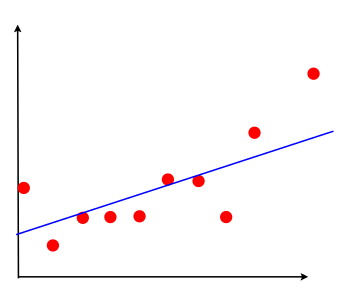
\includegraphics[width=0.6\textwidth, height=5cm]{bias.png}
	\caption[Μοντέλο υψηλής πόλωσης]{Μοντέλο υψηλής πόλωσης}
\end{figure}
Η πρώτη επιλογή μας συνιστά μία ευθεία, δηλαδή ένα πολυώνυμο πρώτης τάξης, το οποίο καθορίζεται από δύο παραμέτρους. Παρατηρούμε πως το μοντέλο αυτό είναι τόσο απλό, που όσο και να προσπαθήσουμε δε θα καταφέρει να προβλέψει καλά τα δεδομένα μας. Θα ήταν ουτοπικό να χαρακτηρίζεται κάποιο πραγματικό φαινόμενο από μια τόσο απλή συνάρτηση, οπότε θα απορρίπταμε αυτό το μοντέλο ως υψηλά πολωμένο, καθώς κάνει μια σημαντική υπόθεση απλότητας.
\begin{figure}[H]
	\centering			
%	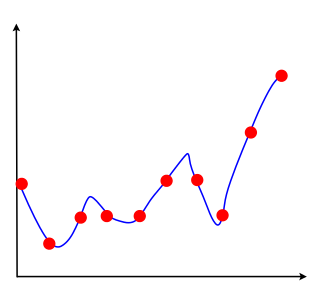
\includegraphics[width=0.6\textwidth, height=5cm]{variance.png}
	\caption[Μοντέλο υψηλής διακύμανσης]{Μοντέλο υψηλής διακύμανσης}
\end{figure}
Η δεύτερη επιλογή μας είναι ένα πολυώνυμο υψηλής τάξης, το οποίο μπορεί εύκολα να επιδείξει μηδενικό σφάλμα στα δεδομένα εκπαίδευσης που διαθέτουμε. Το μοντέλο αυτό είναι φαινομενικά τέλειο και αναπόφευκτα προκαλεί αμφιβολίες: είναι όλα τα δεδομένα μας τόσο αξιόπιστα και χαρακτηριστικά για το φαινόμενο που προβλέπουμε, ώστε να αξίζει να τα προσεγγίσουμε τέλεια; Γενικά, δεδομένα πολύ υψηλής διακύμανσης είναι ύποπτα για θόρυβο, ο οποίος ως τυχαίος είναι συχνά υψίσυχνος, σε αντίθεση με φυσικά δεδομένα που υπακούν σε κάποιες συνθήκες ομαλότητας. Μήπως λοιπόν στην προσπάθειά μας να προβλέψουμε καλά την άγνωστη συνάρτηση παρασυρθήκαμε και μοντελοποιήσαμε το θόρυβο; Ένα τέτοιο μοντέλο είναι καταδικασμένο να αποτύχει σε καινούρια δεδομένα και χαρακτηρίζεται ως μοντέλο υψηλής διακύμανσης. Το παραπάνω πρόβλημα είναι αυτό που έχουμε αποκαλέσει υπερ-προσαρμογή.

Ο θόρυβος, που μας παρασύρει σε υπερ-προσαρμογή, αποτελείται από δύο συνιστώσες: το στοχαστικό θόρυβο, ο οποίος εμφανίζεται τυχαία στα δεδομένα μας και χαρακτηρίζεται από μία κατανομή $\epsilon(x)$ και τον ντετερμινιστικό. Ο τελευταίος οφείλεται στην πολυπλοκότητα της συνάρτηση-στόχου: το μοντέλο ερμηνεύει ως θόρυβο οποιαδήποτε διακύμανση δεν μπορεί να μοντελοποιήσει, καθώς είναι πολύ πολύπλοκη για αυτό, είτε αυτή γεννήθηκε τυχαία είτε προήλθε από τη συνάρτηση-στόχο.

Η μαθηματική αποτύπωση του παραπάνω προβλήματος έχει ως εξής: αν επιλέξουμε ένα μοντέλο $g(x)$ για να προβλέψουμε μια συνάρτηση $f(x)$ και ορίσουμε ως $\bar{g}(x)$ την καλύτερη δυνατή πρόβλεψη που μπορεί να κάνει το μοντέλο δεδομένων των παραμέτρων που περιέχει και της πολυπλοκότητας της $f(x)$ και $g_D(x)$ όλες τις πιθανές υποθέσεις που είναι σε θέση να κάνει το μοντέλο, ρυθμίζοντας τις παραμέτρους του, τότε το σφάλμα στο σετ εκπαίδευσης μπορεί να χαρακτηρισθεί ως εξής:
	\begin{equation}
	E_{error}=\underbrace{E_x(g_D(x) - g(x))^2}_{\text{σφάλμα λόγω  διακύμανσης}} + \underbrace{E_x(\bar{g}(x)- f(x))^2}_{\text{σφάλμα λόγω πόλωσης}} + E_{\epsilon,x}(\epsilon(x^2))
	\end{equation}
\paragraph{Η ιδέα της κανονικοποίησης} Η τεχνική της κανονικοποίησης στοχεύει στη μείωση της διακύμανσης με ταυτόχρονη διατήρηση χαμηλής πόλωσης. Ουσιαστικά προσπαθεί να διατηρήσει την πολυπλοκότητα της υπόθεσης, διατηρώντας το
ίδιο πλήθος παραμέτρων, ώστε να έχει τη δυνατότητα να προβλέψει μια πολύπλοκη συνάρτηση-στόχο, περιορίζοντας ωστόσο την επιλογή των τιμών των παραμέτρων, ώστε να δυσκολεύεται να προβλέψει το θόρυβο.


